










This is also why the naive solution -- strict liability -- fails for platforms. Strict liability causes the platform to internalize the harms from the content it carries, but not the offsetting benefits. Strict liability does not just cause the platform to take down content that is actually harmful. It also causes the platform to remove content that is actually harmless, but which the platform cannot easily distinguish from harmful content. Society, which compares the expected harms $H\lambda(x)$ to the full benefits $s(x)$, is willing to allow content to stay up as long as $lambda(x) \le \frac{s(x)}{H}$. But the platform facing strict liability, which compares the expected harms $H\lambda(x)$ to its lesser private benefits $p(x)$ is willing to allow content to stay up only as long as  $lambda(x) \le \frac{p(x)}{H}$. A platform facing strict liability consistently overmoderates. This overmoderation expresses itself in the removal of harmless content.





Figure~\ref{fig:factory} illustrates social welfare as a function of the factory's output. The net benefit or harm to society from the factory's production at $x$ is given between the signed difference between $p(x)$ and $h(x)$. To the left of the point at which $p$ and $h$ cross, where $p(x) > h(x)$, is net beneficial. Although there are harms from pollution, they are outweighed by the value of the corresponding widgets. Production beyond that point, where $p(x) < h(x)$, is net harmful. Here, the harms from pollution are worse than the value of the corresponding widgets; society would be better off if these widgets were not produced at all. The socially efficient outcome, which we denote $x^e$, occurs when $p(x) = h(x)$. 

The question is how too get there. Consider the following six possible legal regimes:

This is the standard law-and-economics case for strict liability: it is automatically efficient provided that courts can accurately assess the harms caused by the defendant. Negligence and reasonable efforts can also achieve efficiency, but they faces the additional burden of also requiring that the regulator or court chooses the liability threshold correctly. As we will see, one of the essential assumptions of this argument fails for platforms.

%%% XXX Table of liability regimes and factory's marginal profit functions

%%%Instead, free speech law typically follows the negligence strategy of defining an objective standard of care that a reasonable person is expected to follow when acting. One who acts according to that standard of care faces no liability, even if others are harmed. But one who fails to meet that standard is held liable for the resulting harms. In our model, this approach corresponds to defining a threshold of liability $t$ and subjecting the actor to marginal liability:
\begin{equation}
\lt\{\begin{array}{ll}
	0 & \mbox{for $x <t$}, \\
	h(x) & \mbox{for $x \ge t$}.
\end{array}\rt.
\end{equation}


\subsection{Positive Externalities}

A key assumption of the polluting-factory model was that the factory captures all of the social benefit from widget production. There are good reasons to believe that this assumption fails for platforms. In fact, for many platforms it fails twice over.

 Now our factory produces content at a level $\hat{x} \in [0,n]$. As before, it has  marginal profit $p(x)$ and the content causes harms $h(x)$, with the same assumptions on $p(x)$ and $h(x)$. But now we let the positive externalities  of the content be $\delta(x)$, where $\delta(x)$ is weakly decreasing and always positive or zero.\footnote{It may seem artificial to separate $\delta(x)$ and $h(x)$; the reasons will be apparent soon.} We retain the condition that there is still some unambiguously harmful content -- i..e., $h(n) > p(n) + \delta(n)$. The factory's profit function (if it operates) is still 
\begin{equation}
\int_{0}^{\hat{x}} p(x) dx - F
\end{equation}
but now total social welfare is given by
\begin{equation}
\int_{0}^{\hat{x}} p(x) + \delta(x) - h(x) dx - F.
\end{equation}
Now consider the effects of possible regulations.
\begin{itemize}
	\item \textbf{Blanket Immunity}: As above, the factory will set $\hat{x}$ such that $p(\hat{x}) = 0$. But now instead of this \emph{definitely} being overproduction, it is ambiguous. If $h(\hat{x}) > \delta(\hat{x})$, then the factory is overproducing content. But if  $h(\hat{x}) > \delta(\hat{x})$, it will underproduce. If this is efficient, it is fortuitously so.
	\item \textbf{Prohibition}: As above t/k
	\item \textbf{Must-Carry}: As above t/k
	\item \textbf{Strict Liability}: Under strict liability, the factory's marginal profit is $p(x) - h(x)$, so it will produce up to $x^*$ such that $p(x^*) = h(x^*)$. But this is now guaranteed to be underproduction, because the presence of the $\delta(x)$ term now means that $x^e$ is such that $p(x^e) + \delta(x^e) = h(x^e)$.
	 \item \textbf{Negligence}: This regime will be efficient if the regulator sets $t = x^e$.
	 \item \textbf{Reasonable Efforts}: This regime will be efficient if the regulator sets $T$ corresponding to $t$ as above. t/k
\end{itemize}



The difference is that in addition to the platform's revenue $P$, each unit of content that the platform chooses to host also generates an externality of  $\delta \ge 0$ for society at large. Like $P$, we assume that $\delta$ is constant across all content. Thus, while each unit of widget production generates $P$ in marginal profit for the factory, each unit of speech generates $P$ in value for the speaker and $\delta$ in value for society at large, for a total of $P + \delta$.\footnote{We assume that $H < P + \delta$, because otherwise it is socially optimal to maximize speech production, and a blanket immunity is always efficient, even for content known with complete certainty to be harmful.} Now the diagram looks like Figure~\ref{fig:speech}.

\begin{figure}[ht]
	\centering
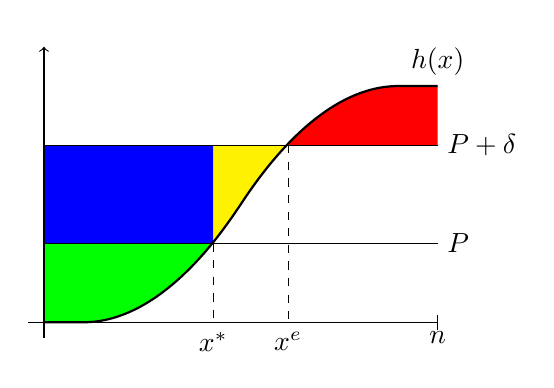
\begin{tikzpicture}[scale=1]
	\fill[green] (0,0) to (.5,0) parabola (2.15,1) to (0,1) to (0,0);
	\fill[red] (3.1,2.25) parabola[bend at end] (4.5,3) to (5,3) to (5,2.25) to (3.1,2.25);
	\fill[blue] (0,1) to (2.15,1) to (2.15,2.25) to (0,2.25) to (0,1);
	\fill[yellow] (2.15,1) parabola bend +(-1.65,-1) (2.5,1.5) parabola bend +(2,1.5) (3.1,2.25) to (2.15,2.25) to (2.15,1);
	\draw[-|] (-0.2,0) -- (5,0) node[below]{$n$}; 
	\draw[->] (0,-0.2) -- (0,3.5) node[above]{};
	\draw[thick] (0,0) to (.5,0) parabola (2.5,1.5) parabola[bend at end] (4.5,3) to (5,3) node[above]{$h(x)$};

	\draw[thin] (0,1) to (5,1) node[right]{$P$};
	\draw[dashed, thin] (2.15,1) -- (2.15,0) node[below]{$x^*$}; 

	\draw[thin] (0,2.25) to (5,2.25) node[right]{$P+\delta$};
	\draw[dashed, thin] (3.1,2.25) -- (3.1,0) node[below]{$x^e$}; 
	
%    \draw[thin] (0,3) to (5,3) node[right]{$S+P+L$};
%    \draw[dashed, thin] (3.55,3) -- (3.55,0) node[below]{$x^e$}; 
	
\end{tikzpicture}
	\caption{Speech Torts}
	\label{fig:speech}
\end{figure}


The efficient level of speech $x^e$ is defined not by where $H\lambda(x)$ intersects the speaker's marginal profit curve $P$ but by where it intersects society's marginal benefit curve $P+\delta$. That is, $x^e$ is such that $\lambda(x^e) = \frac{P+\delta}{H}$, which is strictly greater than $x^e$ in the non-speech case (i.e., where $\delta=0$). So the spillover benefits of speech mean that it is socially optimal to host more speech than in the case where there are no spillovers.

Now consider the liability regimes.
\begin{itemize}
	\item \textbf{Blanket Immunity}: The platform will host all content. This is still inefficient because it includes the net-harmful content at $x > x^e$ (in the red area in Figure~\ref{fig:speech}).
	 \item \textbf{Prohibition}: The platform will host no content. This is still inefficient because it foregoes the net-beneficial content at $x < x^e$ (in the green, blue, and yellow areas in Figure~\ref{fig:speech}). Compared with the non-speech case, prohibition is less likely to be better than blanket immunity, but which is superior depends on $P$, $H$, $\delta$, and $\lambda(x)$.
	 \item \textbf{Strict Liability}: The speaker will produce speech up to $x^*$ where $H\lambda(x^*) = P$. But because $P + \delta > P$ and $\lambda(x)$ is a weakly increasing function, $x^* \le x^e$. Pictorially, the platform will produce up to $x^*$, generating profits in the green region and spillover social benefits in the blue region. But there it will stop, even though the speech from $x^*$ to $x^e$ would have been beneficial to society: the yellow region represents foregone social welfare. Strict liability is strictly better than prohibition, which also gives up the green and blue regions. Whether strict liability is better than full immunity is indeterminate without more constraints on $H$, $P$, $\delta$, and $\lambda(x)$. The yellow region could be larger than the red, or vice versa.
	 \item \textbf{Negligence}: If the negligence threshold is set at $t=x^e$, then the platform's incentives again align with social welfare.\footnote{Cooter, prices and sanctions} Because the threshold is at $x^e$, the platform has no reason not to host content for $x < x^e$. But because $H > P$, any profit the platform makes from hosting content for $x >  x^e$ will be more than outweighed by the damages it must pay. So the platform will stop exactly at $x^e$, the social optimum.
\end{itemize} 
The platform's imperfect information about content is central to these results. If the platform could costlessly distinguish harmless and harmful content, then strict liability would be efficient, as it would be feasible to expect the platform to separate the two and remove only the harmful content. But given imperfect information, the platform \emph{cannot tell with certainty} which content is good and creates positive externalities and which content is harmful and creates negative externalities. 

If the platform is given a legal incentive to remove harmful content, the best it can do is to remove \emph{all} content beyond a threshold of expected harm, which includes both harmful and harmless content.  A strict liability scheme does not take into account the positive spillover benefits to society of harmless content that \emph{from the platform's perspective} is equally likely \emph{ex ante} to be harmful as the harmful content it removes. 

A negligence regime can do better if the regulator can correctly calculate $P$, $\delta$, $H$, and $\lambda(x)$ to set an appropriate threshold. This is not an easy task! If the regulator sets $t$ incorrectly, then any of blanket immunity, strict liability, or negligence could be the most efficient.\footnote{Prohibition is always worse than strict liability, on the assumption that courts correctly calculate $H$. It can be better or worse than blanket immunity or negligence.}




\begin{figure}[ht]
	\centering
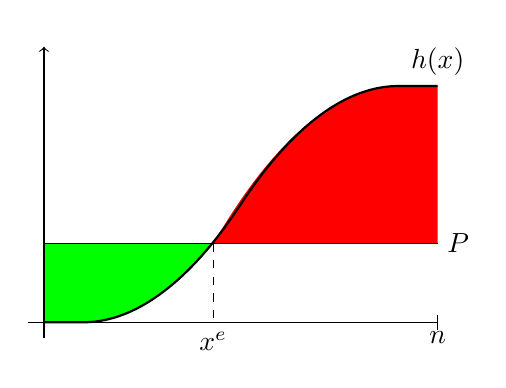
\begin{tikzpicture}[scale=1]
	\fill[green] (0,0) to (.5,0) parabola (2.15,1) to (0,1) to (0,0);
	\fill[red] (2.15,1) parabola[bend at end] (4.5,3) to (5,3) to (5,1) to (2,1);
	\draw[-|] (-0.2,0) -- (5,0) node[below]{$n$}; 
	\draw[->] (0,-0.2) -- (0,3.5) node[above]{};
	\draw[thick] (0,0) to (.5,0) parabola (2.5,1.5) parabola[bend at end] (4.5,3) to (5,3) node[above]{$h(x)$};

	\draw[thin] (0,1) to (5,1) node[right]{$P$};
	\draw[dashed, thin] (2.15,1) -- (2.15,0) node[below]{$x^e$}; 

%    \draw[thin] (0,2) to (5,2) node[right]{$S+P$};
%    \draw[dashed, thin] (1.75,1.5) -- (1.75,0) node[below]{$x^p$}; 
	
%    \draw[thin] (0,3) to (5,3) node[right]{$S+P+L$};
%    \draw[dashed, thin] (3.55,3) -- (3.55,0) node[below]{$x^e$}; 
	
\end{tikzpicture}
	\caption{Non-Speech Torts}
	\label{fig:nonspeech}
\end{figure}

On the one hand, the profit it makes from each additional widget 

The factory earns a constant revenue for each widget it makes. But the more widgets it makes, the greater the probability that each additional widget is defective and harms the consumer who buys it. (For example, the widget-stamping machine might work perfectly at the start of a production run, but gradually deteriorate, so that eventually every widget it makes is defective.) The amount of harm caused by a defective widget is constant, and the factory can tell how likely a widget is to be defective but not which specific widgets are defective, and the factory can and does make the more-likely-to-good widgets first.


We assume that $H > P$.\footnote{In the case where $H \le P$, it is socially optimal for the factory to maximize production, so the only question for a legal regime is how to allocate the costs and benefits of widget production.} Let the probability that a given widget is defective be $\lambda(x)$ for $x \in [0,n]$, where $\lambda(x)$ is a weakly increasing function (i.e. $x < y$ implies $h(x) \le h(y)$). For simplicity of exposition, we assume that some widgets are known to be good (i.e. $\lambda(0) = 0$), and that some widgets are known to be defective (i.e. $\lambda(n) = 1$). 

For example, if $P = \$100$ and $H = \$200$, then $\lambda(\hat{x}) = \frac{1}{2}$, i.e., society is best off if the factory shuts down widget production when exactly half of the widgets coming off the line are defective. At this level of production, every widget the factory produces is likely to be beneficial; every widget it foregoes is likely to be harmful.



\subsection{The Passage of Section 230}

Now we are in a position to appreciate the crucial policy arguments at the heart of Section 230. Famously, Section 230 was enacted against the backdrop of two judicial decisions on the liability of online intermediaries, \emph{Cubby v. Compuserve} and \emph{Stratton Oakmont v. Prodigy}. In \emph{Cubby}, the court held that CompuServe could not be held liable for user-posted content where it "neither knew nor had reason to know" that the content was defamatory.\footnote{Cubby at 141.} But in \emph{Stratton Oakmont}, the court held that Prodigy could be held liable for user-posted content, even where it lacked such knowledge. Both courts treated the cases involving imperfect information -- the issue was how a platform \emph{without} specific knowledge should be treated.

Notoriously, the \emph{Stratton Oakmont} court distinguished \emph{Cubby} on the grounds that Prodigy's "conscious choice, to gain the benefits of editorial control, has opened it up to a greater liability than CompuServe and other computer networks that make no such choice."\footnote{Stratton Oakmont at t/k} On this reasoning, services like CompuServe that exercise no "editorial control" do not face strict liability, whereas moderated services like Prodigy do.

In terms of our model, the rule in \emph{Stratton Oakmont} puts platforms to a choice. If they host \emph{all} content (i.e., set $x^* = n$), they face no liability. But if they moderate \emph{any} content (i.e., set $x^* < n$), they are strictly liable for the harms caused by any content they do not remove.  But such a legal regime creates a powerful incentive not to moderate at all -- indeed, of the two choices, the \emph{Cubby} immunity no moderation at all will always be more profitable than moderation with \emph{Stratton Oakmont} liability. The \emph{Stratton Oakmont} court believed that it was giving Prodigy an incentive to move $x^*$ to the left, closer to $x^e$. But in the presence of the \emph{Cubby} alternative, the Prodigies of the world will be more tempted to move to the opposite extreme, giving up on moderation altogether.

This is why Section 230(c) is titled ``Protection for `Good Samaritan' blocking and screening of offensive material.'' It was enacted to remove the perverse disincentive to moderation created by the rule of \emph{Cubby}. A platform protected by Section 230 is now free to move $x^*$ off the right endpoint without fear that it will now open itself to liability and be forced to move much further to the left. It might do so out of civic-mindedness, to reduce public-relations trouble, or (as Prodigy did) to create a better experience for users.\footnote{A downward-sloping $P$ curve that crosses the $x$ axis would capture these motivations.}




\subsection{Section 512}

A model in which the platform can optionally investigate content sheds light on the controversies over the notice-and-takedown regime of Section 512 of the Copyright Act. The basic rule of Section 512 is that a hosting platform ``shall not be liable for monetary relief \ldots for infringement of copyright by reason of the storage at the direction of a user of [infringing] material.''\footnote{17 U.S.C. § 512(c)(1).} This is a blanket immunity, but it is qualified by five (!) exceptions.

First, Section 512(c)(1)(A)(i) removes the platform's immunity as to specific material if it has ``actual knowledge that the material \ldots is infringing''\footnote{17 U.S.C. § 512(c)(1)(A)(i).} and the platform does not ``act[] expeditiously to remove, or disable access to, the material.''\footnote{17 U.S.C. § 512(c)(1)(A)(iii).} One way of looking at this exception is that reflects the intuition that where the platform \emph{has} performed an investigation into specific content, it can remove harmful items without affecting non-harmful items. It does not matter where along the $\lambda(x)$ curve the item falls -- the point is that once the platform has knowledge, it must act. 

Second, Section 512(c)(1)(A)(ii) removes the platform's immunity as to specific content if it is ``aware of facts or circumstances from which infringing activity is apparent'' and fails to remove the content.\footnote{17 U.S.C. § 512(c)(1)(A)(ii).} This exception, known in the caselaw and scholarship as the ``red flag'' provision, is best understood as a judgment that in certain cases, the probability of infringement is high enough to justify removal. In other words, the red flag provision is a negligence-style rule: beyond some threshold $t$ of high likelihood that content is infringing, the platform will be liable for all such infringing content. Caselaw confirms that $t$ is high. It is not enough that the platform is aware in general that some content is infringing; it must be awareness of ``facts that would have made the specific infringement `objectively' obvious to a reasonable person.''\footnote{Viacom v. YouTube at 31.} 

Third, Section 512(c)(1)(B) removes the platform's immunity if it ``receive[s] a financial benefit directly attributable to the infringing activity, in a case in which the service provider has the right and ability to control such activity.''\footnote{17 U.S.C. § 512(c)(1)(B).} This standard, which resembles but is not identical in application to the common-law vicarious-infringement standard,\footnote{Reese} is not in theory tied to the platform's knowledge at all. Instead, it is designed to smoke out situations in which a platform that could block infringement has especially bad incentives to turn a blind eye to it. In terms of our model, we think these are situations in which $c$ is small (so that the platform has the ``ability to control'' infringement) and $P$ is large (so that the platform has strong private incentives to allow as much infringement as it can). These are circumstances under which in the absence of liability, the platform might under-invest in investigating likely-to-be-infringing content.

Fourth, Section 512(c)(1)(C) removes the platform's immunity if it receives a ``notification of claimed infringement'' and fails to remove it.\footnote{17 U.S.C. § 512(c)(1)(C).} The value of a takedown notice is that it reduces the investigation costs as to specific content by narrowing the issues the platform must investigate. When investigation is expensive, as we have seen, a rational platform will not bother searching for the needle -- instead, it will overmoderate and throw out the entire haystack. But when someone points to an alleged needle, it is far easier for the platform to decide whether it is actually a needle.

Here, it is helpful to drill down on what exactly the investigation costs $c$ consist of in the case of copyright infringement.  A claim of copyright infringement requires proof that (1) particular material (2) uses a copyrighted work (3) in a way that infringes. In the abstract, investigation is expensive because a platform must investigate all of its content, compare that content to all copyrighted works, and consider all possible justifications (such as licenses, fair use, etc.).  The statutory template for a takedown notice addresses these elements by requiring, respectively, ``[i]dentification of the material that is claimed to be infringing \ldots and information reasonably sufficient to permit the service provider to locate the material.''\footnote{17 U.S.C. § 512(c)(3)(A)(iii).}, ``[i]dentification of the copyrighted work claimed to have been infringed,'',\footnote{17 U.S.C. § 512(c)(3)(A)(ii).}, and ``[a] statement that the complaining party has a good faith belief that use of the material \ldots  is not authorized by the copyright owner, its agent, or the law.''\footnote{17 U.S.C. § 512(c)(3)(A)(v).}

Experience has shown that these three requirements stand on somewhat different footing. Courts have generally been unwilling to relax the requirement of identification of specific material, recognizing that without that specific identification the platform must investigate a vast array of content.\footnote{Perfect 10, etc.} And plaintiffs have also been held to the requirement that they identify the relevant copyrighted works. (Indeed, in a world where copyright subsists on fixation, almost every upload will contain material that is copyrighted by someone, so that all of the important questions about the copyright itself go to whether the uploader had the right to do so.) But courts have held that the ``good faith belief'' required by Section 512(c)(3)(A)(v) can be satisfied by a subjective belief, regardless of whether that belief is reasonable or not -- and even if the notice-sender acts in bad faith, the damages against them are likely to be nominal at best.\footnote{Rossi, Lenz}

This leniency by courts undermines the point of the notice-and-takedown rule. The point of a Section 512 notice is that it is a \emph{signal}. The platform can forego the required investigative costs $c$ because the notice sender has either borne them itself or is in a position to investigate more cheaply because it has more access to the relevant information. \footnote{In the same way, the counter-notice-and-putback provisions of Section 512(g) are intended to act as a signal by the uploader, who can credibly signal that the material is not infringing.} But if the penalty the sender must pay for sending a false or mistaken takedown notice is minimal, many copyright owners will rationally conclude that they are better off sending takedown notices aggressively, even in cases that are highly unlikely to infringe -- degrading the signal and pushing the investigative costs back onto the platform. 

The result, predictably, is overmoderation. A platform will investigate noticed content rather than simply take it down  only if its potential profit from hosting the content is greater than the cost of doing an investigation, i.e. if $P > c$. For a video that might generate a few cents in ad revenue but would take several dollars of employee time to review, takedown is the preferred response. 

But there is more. If the signal of an infringement notice is too weak, the platform \emph{will not even investigate}; it will leave the material up. We have been acting as though a notice gives certainty of infringement. But if all it does is adjust the platform's estimate $\lambda(x)$ of the likelihood of infringement, it could be that $H\lambda(x) < c$. And if that is the case, the notice-and-takedown system will collapse entirely, because a notice is no longer an effective signal of infringement. It does not appear that this is the case under the present Section 512, but a notice-and-takedown system that does not impose sufficient safeguards fails to make a notice a credible signal of harmfulness to induce platforms to take action.

Fifth and finally, under Section 512(i) to be eligible for the safe harbor at all, a platform must ``adopt[] and reasonably implement[] \ldots a policy that provides for the termination in appropriate circumstances of \ldots repeat infringers.''\footnote{17 U.S.C. § 512(i)(1)(A).} This repeat-infringer-policy (R.I.P.) requirement has a different structure than exceptions discussed above. Those exceptions apply to \emph{specific content} that the platform fails to remove. But the R.I.P. requirement is a threshold. If a platform doen't do a good enough job at removing content posted by repeat infringers, it is not eligible for the safe harbor \emph{at all}, even for material posted by others. This is a different kind of liability rule, and it is worth modeling separately. 

Formally, under a \textbf{Conditional Immunity} regime \ldots details t/k.

To summarize, the five limitations on the Section 512(c) safe harbor all function in different ways, and they all have to do with investigative costs. The actual-knowledge provision deals with cases where $c = 0$ and no investigation is required; the red-flag provision deals with cases where $\lambda(x)$ is high and the content is likely to infringe; the financial-benefit provision deals with cases where $c$ is low and $P$ is high so the platform has bad incentives not to investigate; the notice-and-takedown provision deals with cases where the copyright owner has taken on the investigative costs $c$ itself; and the R.I.P. provision t/k summarize.

Another way of looking at these exceptions is from the perspective of what society \emph{wants} a platform do to. In terms of our model, a regulator's ideal is that a platform will (1) remove all infringing content at or above $\underline{x^e}23$, (2) leave up all non-infringing content at or below $\overline{x^e}$, (3) investigate only in cases between $\underline{x^e}$ and $\overline{x^e}$ where it is cost-justified to do so, and (4) remove infringing content, even below $\underline{x^e}$, in cases where someone else has done the investigation more efficiently. The design of the Section 512(c) conditions reflects an imperfect attempt to achieve these goals.




% \subsection{Model 3: Imperfect Information About Speech}



% But now we add a second dimension: each item of content is a pair $(x,y)$.  The $x$ axis measures harmfulness $h(x)$, as before. But the $y$ axis, which ranges from $0$ to $m$, measures the \emph{fraction} of content that is harmful. That is, for content at $(x,y)$, a fraction $\lambda(y)$ of that content is harmful and generates harm $h(x)$ per unit and a fraction $ 1- \lambda(y)$ is harmless and generates $0$ harm. The speaker of an item of content knows whether it is harmful or not, as does the regulator, but the platform does not. Instead, the platform observes the \emph{probability} $\lambda(y)$ that the item is harmful, where $\lambda(y)$ is a weakly increasing function of $y$, with $\lambda(0) = 0$. That is, the harmfulness $h(x,y)$ of content $(x,y)$ is given by:
% \begin{equation}
% h(x,y)=
% \lt\{\begin{array}{ll}
%     h(x) & \mbox{with probability $\lambda(y)$}, \\
%     0 & \mbox{with probability $1 - \lambda(y)$}.
% \end{array}\rt.
% \end{equation}
% In expectation, a unit of content at $y$ will generate harm $\lambda(y)h(x)$. Start by examining the platform's incentives. Hold $x$ fixed (so that $h(x)$ is constant and consider the following diagram of benefits and harms as as a function of $y$:
% \begin{figure}[h]
%     \centering
% \begin{tikzpicture}[scale=1]
% %    \fill[green] (0,0) to (.5,0) parabola (2.15,1) to (0,1) to (0,0);
% %    \fill[red] (3.1,2.25) parabola[bend at end] (4.5,3) to (5,3) to (5,2.25) to (3.1,2.25);
% %    \fill[blue] (0,1) to (2.15,1) to (2.15,2.25) to (0,2.25) to (0,1);
% %    \fill[yellow] (2.15,1) parabola bend +(-1.65,-1) (2.5,1.5) parabola bend +(2,1.5) (3.1,2.25) to (2.15,2.25) to (2.15,1);
%     \draw[-|] (-0.2,0) -- (5,0) node[below]{$m$}; 
%     \draw[->] (0,-0.2) -- (0,3.5) node[above]{};
%     \draw[thick] (0,0) to (.5,0) parabola (2.5,1.5) parabola[bend at end] (4.5,3) to (5,3) node[above]{$\lambda(y)h(x)$};

%     \draw[thin] (0,1) to (5,1) node[right]{$P$};
%     \draw[dashed, thin] (2.15,1) -- (2.15,0) node[below]{$y^*$}; 

%     \draw[thin] (0,2.25) to (5,2.25) node[right]{$P+S+\delta$};
%     \draw[dashed, thin] (3.1,2.25) -- (3.1,0) node[below]{$y^e$}; 
	
% %    \draw[thin] (0,3) to (5,3) node[right]{$S+P+L$};
% %    \draw[dashed, thin] (3.55,3) -- (3.55,0) node[below]{$x^e$}; 
% \end{tikzpicture}
%     \caption{Speech Torts with Imperfect Information}
%     \label{fig:speechimperfect}
% \end{figure}
% Observe that the curve $\lambda(y)$ has \emph{exactly the same shape} as $h(x)$ did in the previous diagram. We have replaced a deterministic but variable harm $h(x)$ with a probabilistic but fixed harm $\lambda(y)h(x)$. This means that the analysis from the previous model carries over: if the platform chooses to allow content $y$ to remain up, it generates private value $P$ per unit, social value $P+S+\delta$ per unit, and \emph{expected} harm $h(x,y) = \lambda(y)h(x)$ per unit. As long as the platform's potential liability is a weakly increasing function in $y$, it will choose a threshold $\hat{y}$ that maximizes its profits by taking down all content $y > \hat{y}$ beyond the threshold and leaving up all content $y \le \hat{y}$. And as before, there is a socially efficient choice $y^e$, determined by $\lambda(y^e) = \frac{P + S+ \delta}{H}$, at which the platform takes up all and only that content whose expected harms exceed its social value. 

% As before, complete immunity leads to undermoderation because the platform sets $\hat{y} = m$, allowing expected net-harmful content to remain. Prohibition leads to overmoderation because the platform sets $\hat{y} = 0$, taking down expected net-beneficial content. Strict liability leads the platform to overmoderate (although less than for prohibition) because the platform sets $\hat{y} = y^{\ast}$ defined by $\lambda(y^{\ast} = \frac{P}{H})$, and $y^{\ast} \le y^e$. Threshold liability is efficient when the threshold is set at $y^e$. The regulator takes into account the value to speakers and society at large of speech.

% What is different about this model is that the \emph{platform}'s incentives are different than the \emph{speaker}'s. In particular, because speakers have perfect information along the $y$ axis about whether their content is harmful or not, they have an option the platform does not: to omit the harmful speech while still producing the harmless speech. Because the platform only observes $\lambda(y)$, a noisy signal of the speech's harmfulness, it must remove both harmful and harmless content that have the same $\lambda(y)$.

% Observe that \emph{along the $x$ axis of harmfulness}, the regulator's optimal behavior towards speakers \emph{is unchanged}. Strict liability is inefficient in the range $S < h(x) < P + S + \delta$, but threshold liability at $x^e$ defined by $h(x^e) = P + S + \delta$ is socially optimal. The regulator takes into account the value to the platform and to society at large.

% In other words, \emph{platform immunity rests on a related but distinct basis than speaker protections}. Both of them depend on positive externalities: when $\delta = 0$, the argument for a more speech-protective regime than strict liability collapses. But the pure speaker-protective argument is that some speech is valuable \emph{notwithstanding} the harms it causes, while the platform-protective argument is that some valuable speech is \emph{indistinguishable} from harmful speech.

% There are also good reasons to believe that in typical cases, the value $P$ extracted by a platform is significantly smaller than the value $S$ realized by the users who post content. Estimates of the net social utility created for platform users vastly exceed estimates of the platforms' revenues. This means that in practice, platforms have significantly weaker private incentives to host speech than orignal speakers do. Strict liability more significantly deters platforms than speakers.

% This is a standard argument for treating speech torts differently than other types of torts. Because the speaker creates value for listeners and for society by spreading information, the value of the speech \emph{to them} must be weighed against the harm that it causes. Thus, harmful true speech is frequently protected (e.g. negative consumer reviews). Similarly, the public-disclosure tort contains a First-Amendment-driven exception when the information is of legitimate public concern, i.e., when $\delta$ is high. 



% This model explains why speech law is more solicitous of speakers than of other actors. But notice that it cannot yet explain why speech law is even more solicitous of platforms than it is of speakers! The spillover critique of strict liability applies just as strongly to original speakers as it does to platforms. And the negligence strategy suggests that the threshold of liability should be based entirely on the overall \emph{social} costs and benefits of the speech: whatever that threshold is, it should apply equally to speakers and platforms, regardless of their private incentives. Something further is required to make sense of platform immunity.
